% ##################################################################################################################
\section{Quito Metropolitan District, Ecuador}
\label{sec:quito}
\hfill \textbf{Author:} Rolando Armas, Hernán Aguirre

% ##################################################################################################################
Quito Metropolitan District - DMQ (Ecuador) has grown rapidly the last years increasing traffic congestion, gas emissions, pollution, and use of energy. Our research integrates evolutionary computation, traffic simulation, emission models, and data mining tools to gain a better understanding on DMQ’s complex mobility and transportation system and propose solutions to it from a sustainability standpoint.

As a first case study \citep[][]{ArmasEtAl_SEAL_2014}, we have implemented a mobility scenario to optimize traffic lights under congested conditions. We have focused on the
DMQ’s business district, which geographical area covers 7x3\,square kilometers as shown in Figure~\ref{fig:fig1}. The area considers only the primary and secondary pathways, which free speeds are in the range from 30 to 80\,kilometers per hour. The network has 1\,000\,links approximately and comes from Geofabrik and OpenStreetMap. The number of simulated agents is 20\,000. The mobility plan for each agent consists of three main trips: (1) home to work, (2) work to leisure, and (3) leisure to home (see Figure~\ref{fig:fig2}). The plans are designed so that all agents move first from south to north, completely crossing the geographical area of study. In their second trip, the agents move from north to the central zone of the area under study and in their last trip from the central zone to the south. Eleven signal lights are located in a main two-way street with flows in south-north and north-south directions (see Figure~\ref{fig:fig1}).

The evolutionary algorithm finds optimal signal settings of the DMQ scenario minimizing average travel time. First, we run MATSim for 500\,iterations, making sure it reaches a user equilibrium state without setting any traffic signal. After that, the evolutionary algorithm evolves a population of candidate solutions for a number of generations. Each solution represents a configuration of signals (signal control) for the transportation system. At each generation, the evolutionary algorithm calls MATSim for each candidate solution in order to evaluate it. MATSim starts from the equilibrium state setting its signals controls with the tentative solution provided by the optimizer and runs one additional iteration. The output collected from that iteration of the simulator is used to calculate travel time, which is passed as fitness of the solution to the optimizer. Figure~\ref{fig:fig2} illustrates the interaction of MATSim and the evolutionary algorithm. The first case study \citep[][]{ArmasEtAl_SEAL_2014} provides valuable insights to understand better the optimal setting of traffic lights in the business district of DMQ under congested conditions, allows us to validate the problem representation used in the evolutionary algorithm and the effectiveness of the mutation and recombination operators implemented to search solutions.

Currently, we are scaling up the number of traffic signals to be optimized and testing under other mobility scenarios within the same area of study. Our next step is to incorporate a emissions model and use multi- and many-objective evolutionary algorithms \citep[][]{AguireEtAl_EMO_2013} to evolve optimal designs of the transportation and mobility system of the DMQ satisfying multiple criteria for sustainability. These criteria include desired transportation and mobility policies, accessibility, reduction of emissions, reduction of energy use, and societal and economic benefit.

\createfigure%
{Area of study}%
{Area of study}%
{\label{fig:fig1}}%
{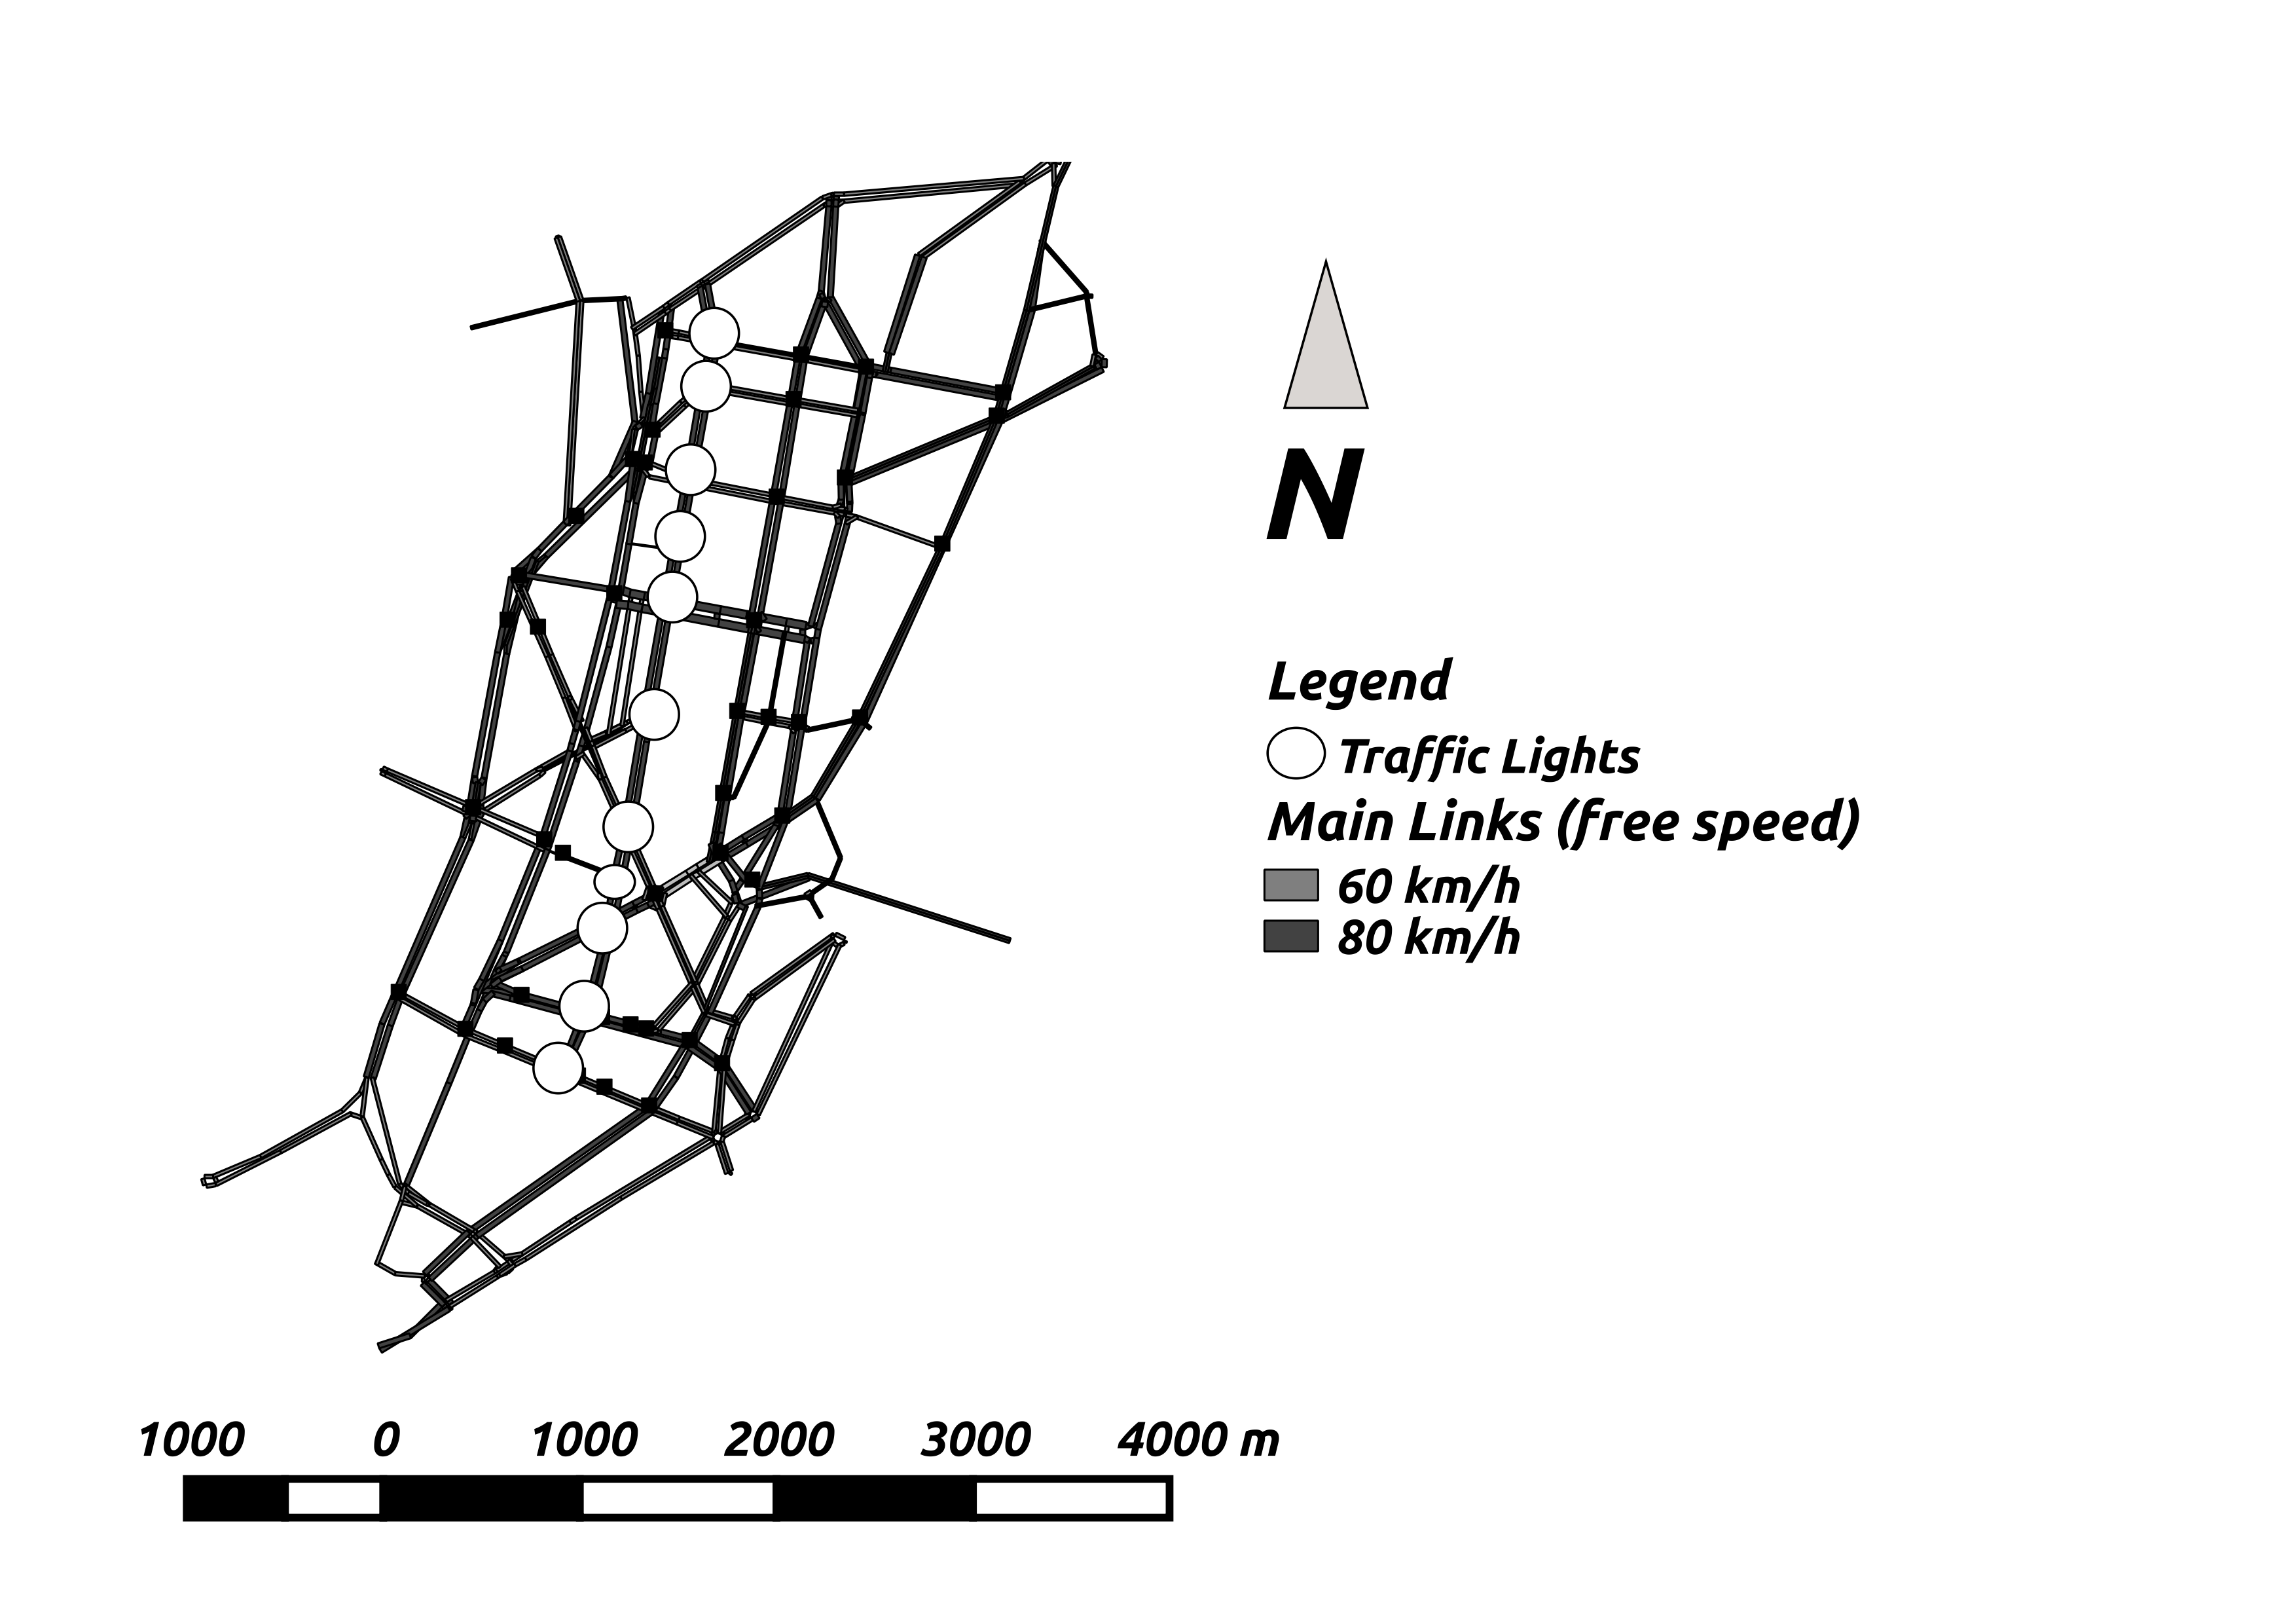
\includegraphics[width=0.7\textwidth, angle=0]{./using/figures/qfig1.png}}%
{}

\createfigure%
{Optimization system}%
{Optimization system}%
{\label{fig:fig2}}%
{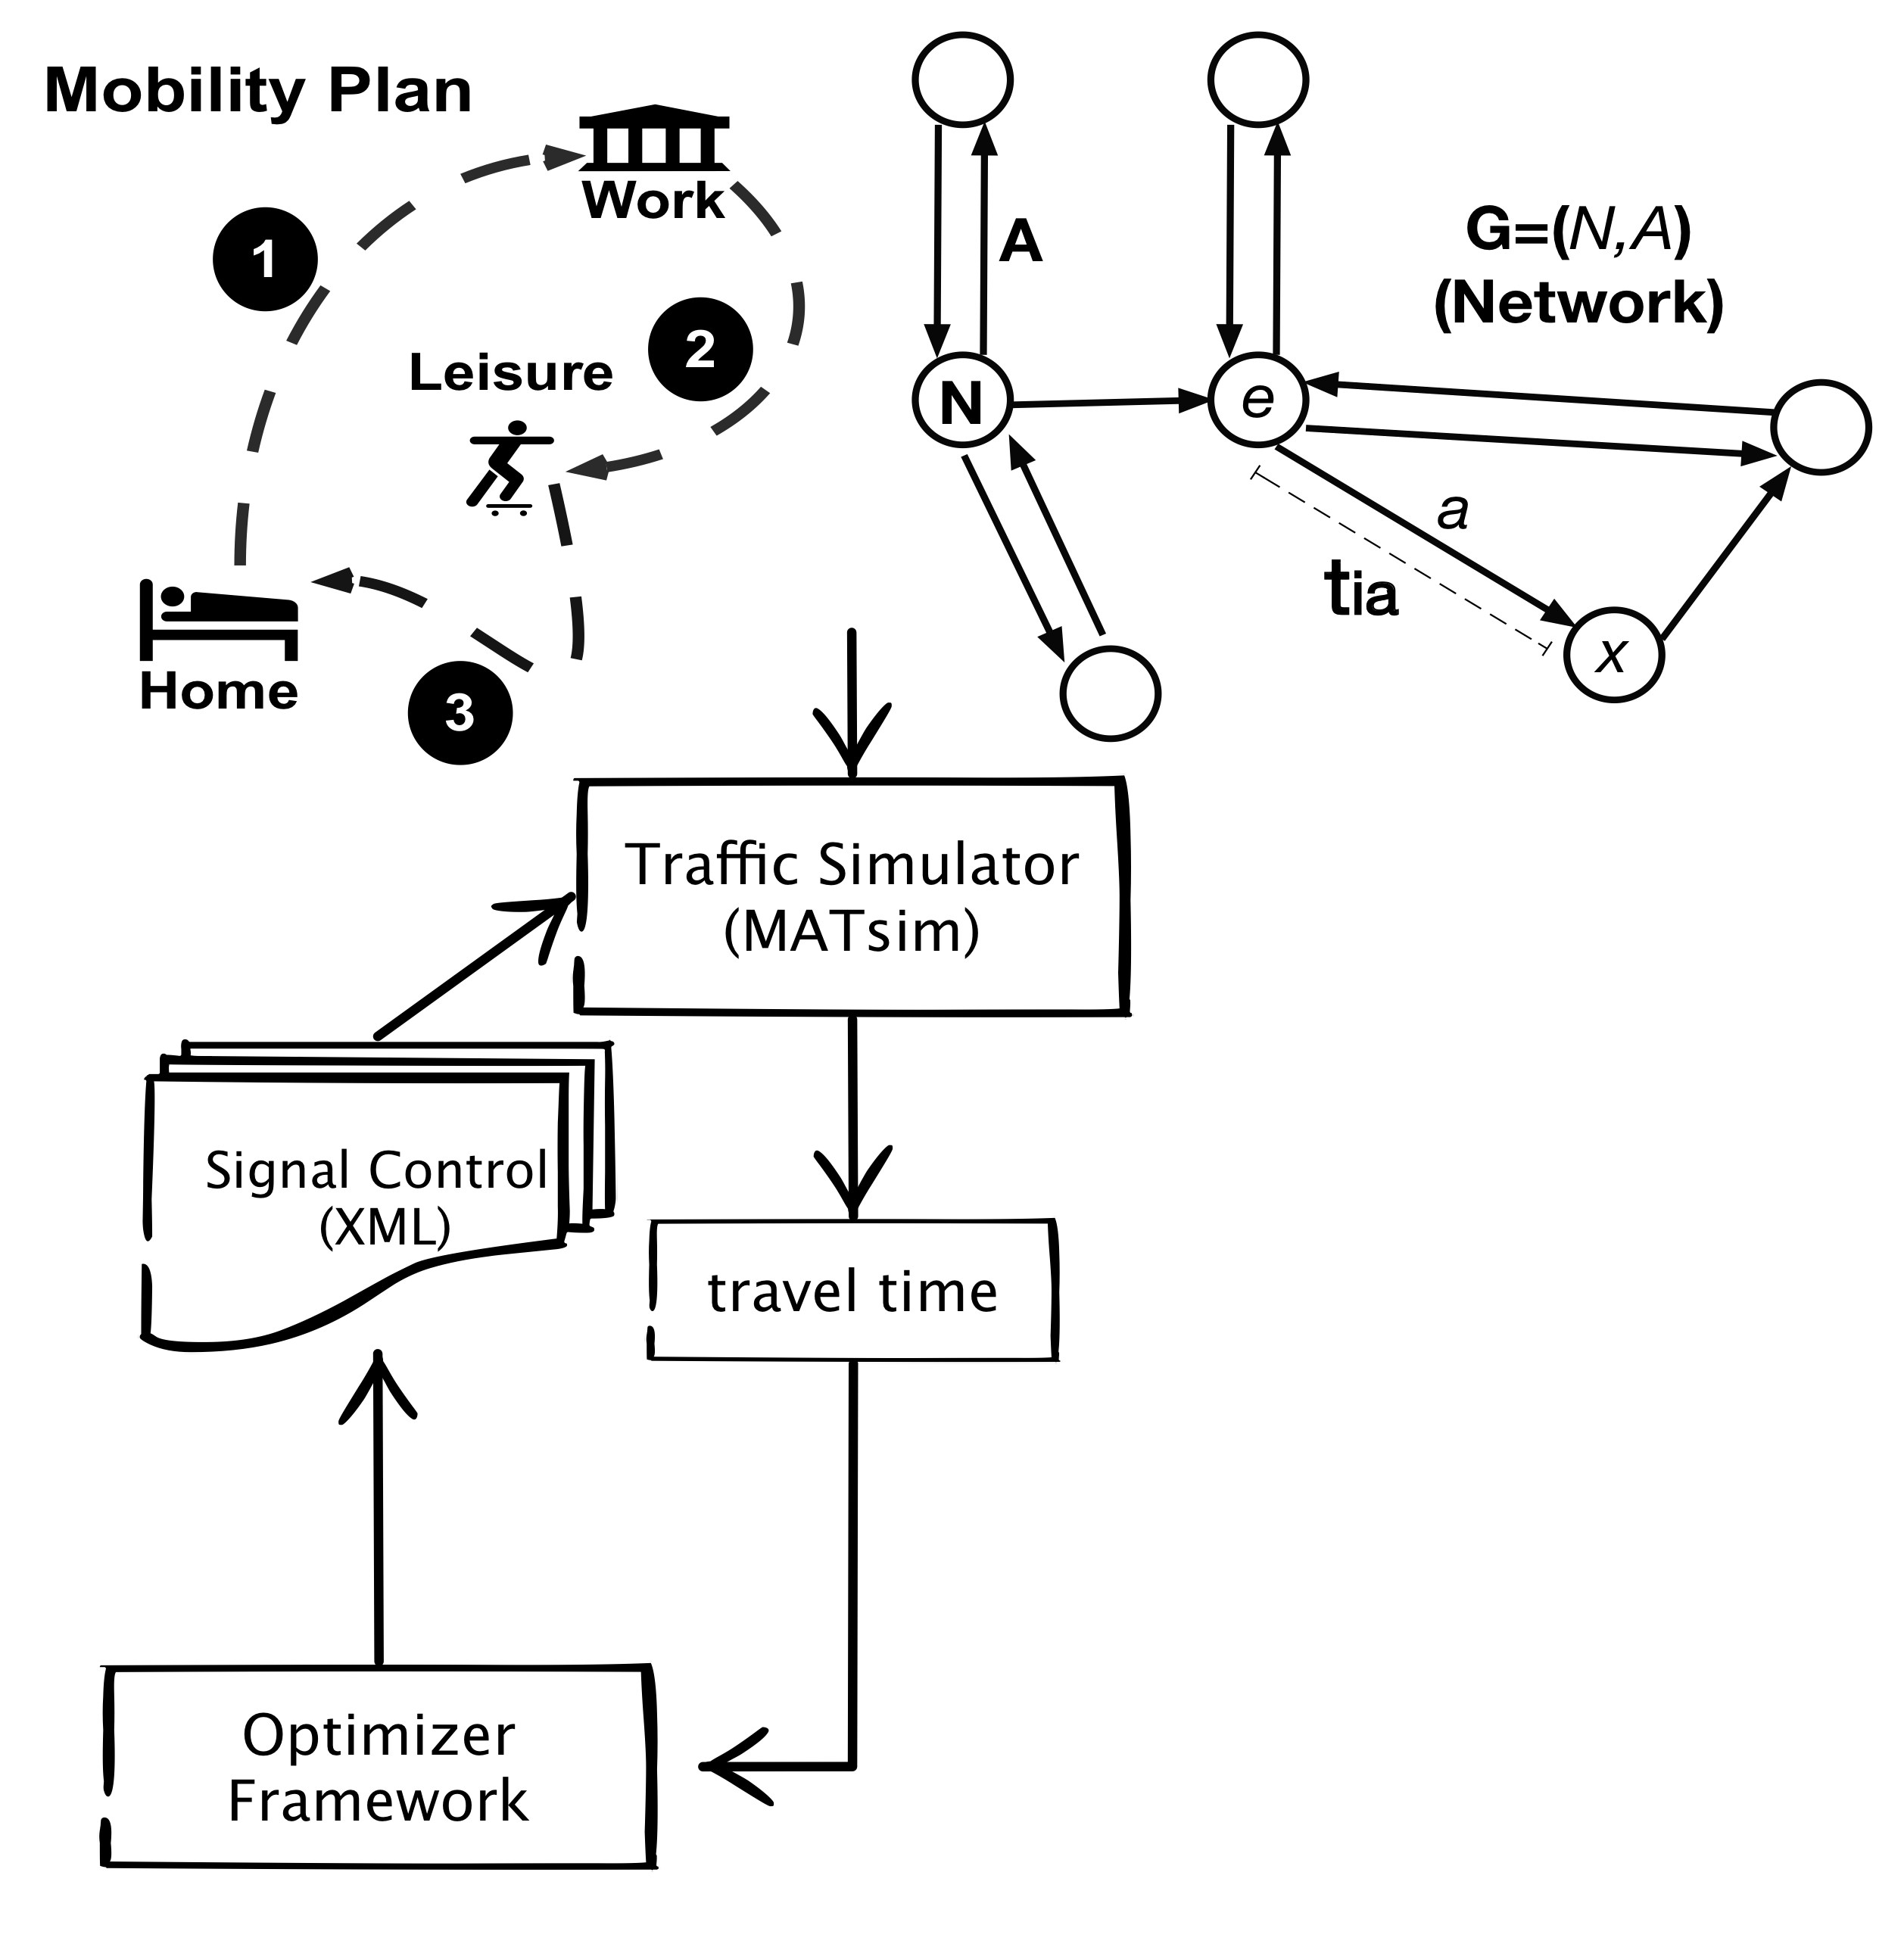
\includegraphics[width=0.7\textwidth, angle=0]{./using/figures/qfig2.png}}%
{}

% ##################################################################################################################


